\section{Experiments \& Results}

\subsection{Part 1 Results: Hopper Continuous Control}

All three algorithms were trained for 70{,}000 episodes on the Hopper-v4 environment, repeated across three independent seeds.
Table~\ref{tab:part1_results} summarises the training performance;
Figure~\ref{fig:experiments_reward} shows the learning curves (rolling average over 100 episodes $\pm$ standard deviation across seeds).


\begin{table}[ht]
\centering
\caption{Training performance on Hopper-v4 (mean over 3 seeds). \emph{Avg-100} denotes the 100-episode rolling mean return. \emph{Std} and \emph{Avg Ep.\ Len} are computed over all $70{,}000$ training episodes.}
\label{tab:part1_results}
\resizebox{\linewidth}{!}{%
\renewcommand{\arraystretch}{1.05}
\begin{tabular}{lrrrrcc}
\hline
\textbf{Algorithm} & \textbf{Best Avg-100} & \textbf{Final Avg-100} & \textbf{Std} & \textbf{Best Episode} & \textbf{Avg Ep.\ Len} & \textbf{Time (min)} \\
\hline
REINFORCE ($b{=}0$)  & 1006 & 635  & 257 & 2811 & 178 & 57.6 \\
REINFORCE ($b{=}20$) & 1807 & 806  & 399 & 3152 & 215 & 70.3 \\
Actor-Critic         & \textbf{1938} & \textbf{1360} & \textbf{734} & \textbf{3480} & \textbf{249} & \textbf{83.8} \\
\hline
\end{tabular}%
}
\end{table}

\begin{table}[ht]
\centering
\caption{Test return (mean $\pm$ std) on Hopper-v4, per seed.}
\label{tab:part1_test_results}
\resizebox{\linewidth}{!}{%
\renewcommand{\arraystretch}{1.1}
\begin{tabular}{lccc}
\hline
\textbf{Algorithm} & \textbf{Seed 1} & \textbf{Seed 2} & \textbf{Seed 3} \\
\hline
REINFORCE ($b{=}0$)  & $710 \pm 484$ & $726 \pm 296$ & $1305 \pm 547$ \\
REINFORCE ($b{=}20$) & $782 \pm 929$ & $1461 \pm 1097$ & $2444 \pm 182$ \\
Actor-Critic         & $1725 \pm 1382$ & $\mathbf{3335 \pm 14}$ & $760 \pm 111$ \\
\hline
\end{tabular}%
}
\end{table}

\begin{figure}[ht]
    \centering
    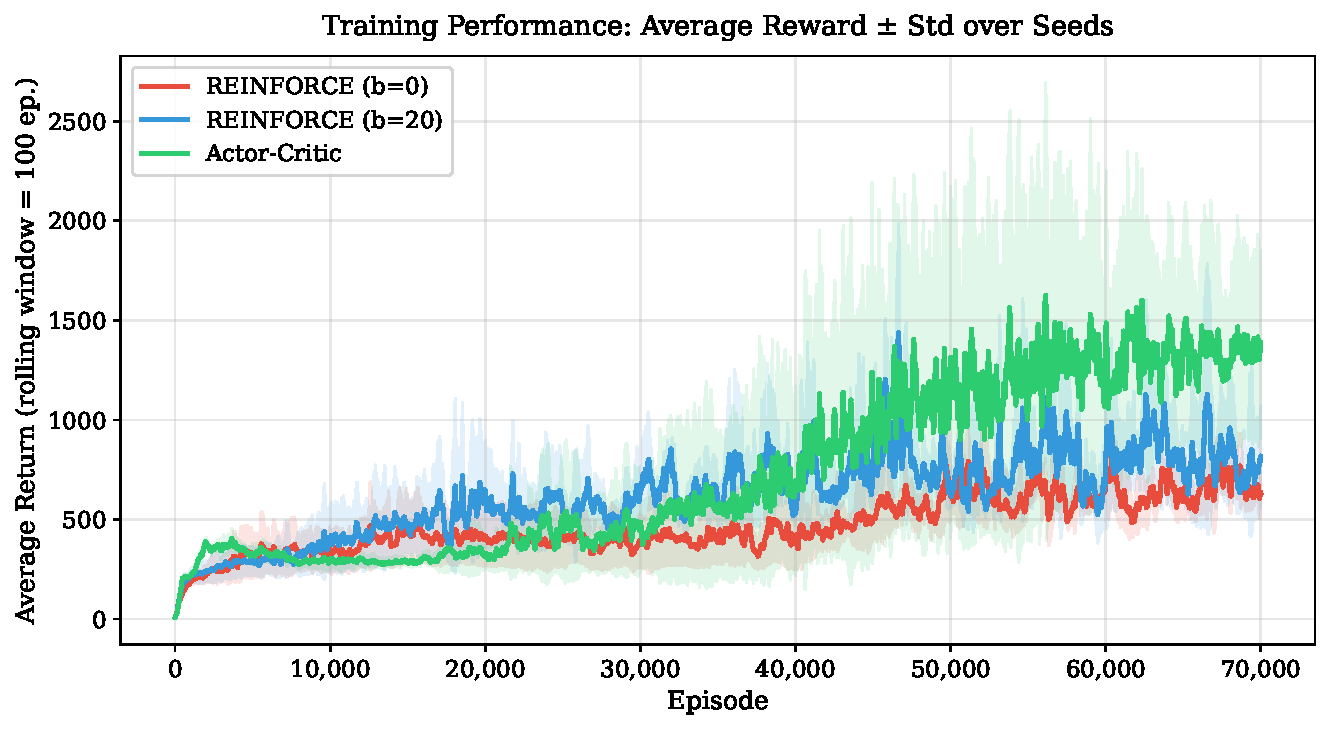
\includegraphics[width=0.8\linewidth]{imgs/experiments_reward.pdf}
    \caption{Average return (rolling window $= 100$ episodes) $\pm$ standard deviation across 3 seeds for REINFORCE ($b{=}0$, $b{=}20$) and Actor-Critic on Hopper-v4.}
    \label{fig:experiments_reward}
\end{figure}

As we can clearly see from Table~\ref{tab:part1_results}, the Actor-Critic achieved the best overall training performance, outperforming the other models 
in terms of highest Best Avg-100 reward, highest Final Avg-100 reward, highest Best Episode reward and longest average episode length.
In turn, REINFORCE with baseline achieved better overall scores than vanilla REINFORCE, improving both the Best Avg-100 reward and the average
episode length.
Interestingly, despite expecting a gradient-estimator variance reduction with the introduction of a baseline, the opposite behaviour was recorded,
where REINFORCE with baseline exhibited a higher reward standard deviation than vanilla REINFORCE.

Figure~\ref{fig:experiments_reward} shows that the Hopper improved its policy throughout training under all algorithms.
However, the Actor-Critic achieved faster policy improvement, reaching larger rewards more quickly and eventually reaching reward scores that neither of the REINFORCE
variants were able to obtain.

The test results reported in Table~\ref{tab:part1_test_results} support the claim that the Actor-Critic outperformed the other approaches, although substantial variability
across seeds was recorded.
Indeed, the best Actor-Critic seed achieved a mean test return of $3335 \pm 14$ and consistently survived for the full episode.
On the other hand, the worst seed achieved a mere $760 \pm 111$ reward score, proving that Actor-Critic did not perform consistently across different seeds.
Lower scores but similar variability was observed for both REINFORCE variants.

Overall, the Actor-Critic performed the best both in training and testing among the evaluated methods.
Nevertheless, the large differences between seeds indicate that learning remained sensitive to initialization and stochastic training effects.












\subsection{Part 2 Results: PandaPush Sim-to-Sim Transfer}
Table \ref{tab:sim2real_results} shows the performance of the evaluated algorithms across different train and test configurations. 
As a baseline, PPO failed to consistently solve the task even on the source environment, plateauing at a mean return of -3.485. In contrast, SAC successfully learned the pushing behavior.

To evaluate the sim-to-real transfer, we established a lower bound using vanilla SAC trained on the source and tested on the target environment, which achieved a return of -0.633. The upper bound was established by training and testing SAC directly on the target environment, yielding a return of -0.445. 

The reality gap is evident in the performance drop of vanilla SAC. 
Applying domain randomization successfully mitigated this gap. While ADR improved the transfer return, 
UDR achieved the best overall transfer performance as seen in Table \ref{tab:sim2real_results}.
Relative to the upper bound, UDR successfully closed approximately 66\% of the reality gap while maintaining a very high success rate.

\begin{table}[h]
\centering
\resizebox{\columnwidth}{!}{%
\begin{tabular}{lcccc}
\hline
\textbf{Algorithm \& Strategy} & \textbf{Train Env} & \textbf{Test Env} & \textbf{Mean Return} & \textbf{Success Rate} \\ \hline
PPO (Vanilla) & Source & Source & $-3.485 \pm 0.091$ & $20.0\% \pm 0.1\%$ \\
SAC (Vanilla) & Source & Source & $-0.565 \pm 0.118$ & $98.5\% \pm 2.1\%$ \\
SAC (Vanilla) - Lower Bound & Source & Target & $-0.633 \pm 0.152$ & $97.5\% \pm 3.5\%$ \\
SAC + UDR & Source & Source & $-0.485 \pm 0.036$ & $99.5\% \pm 0.4\%$ \\
SAC + ADR & Source & Source & $-0.583 \pm 0.079$ & $98.3\% \pm 1.2\%$ \\
SAC + ADR & Source & Target & $-0.556 \pm 0.044$ & $99.2\% \pm 0.8\%$ \\
SAC + UDR - Best Transfer & Source & Target & $-0.509 \pm 0.032$ & $99.7\% \pm 0.2\%$ \\
SAC (Oracle) - Upper Bound & Target & Target & $-0.445 \pm 0.019$ & $100.0\% \pm 0.0\%$ \\ \hline
\end{tabular}%
}
\caption{Performance comparison across training strategies and evaluation domains (mean $\pm$ std over 3 seeds, 200 episodes per seed).}
\label{tab:sim2real_results}
\end{table}
